\chapter{Background}
\label{ch:background}

\blockquote{The focus of this chapter is to explain the concept of lexical flexibility, consider its criticisms, and offer a more robust, functionally-grounded definition instead. I first briefly describe how flexible approaches to lexical categories developed as a response to weaknesses in traditional theories of parts of speech. I then survey the landmark studies and important findings on lexical flexibility, along with criticisms of this research. Following that, I summarize approaches to lexical categories from several functionalist perspectives—cognitive linguistics, typology, and construction grammar. I conclude by offering a revised formulation of lexical flexibility which is more in line with this functional research.}

\section{Introduction: Approaches to lexical flexibility}
\label{sec:2.1}

The field of linguistics as a whole, and the subfield of typology in particular, is undergoing a radical shift in how we understand lexical categories, along primarily two dimensions. The first dimension is our understanding of what lexical categories are a property \emph{of}. Early researchers viewed categories as universal properties of both language and languages \addcite{Haspelmath on g-language vs. p-language; add these terms in parentheses}. I call this the \dfn{universalist} position. After Boas, many researchers then came to view categories as language-specific, with patterned similarities across languages. I call this the \dfn{relativist} approach. Most recently, some researchers view categories as typological patterns rather than properties of any particular language. This is the \dfn{typological} position, and the one I adopt here.

The second dimension of historical change in linguistic theories of categories is in the \emph{nature} of the categories themselves. In the Classical tradition, categories were thought to be categorical and well-defined by a set of necessary and sufficient conditions (in the tradition of Aristotle). After the cognitive turn in the 1980s, many linguists came to view categories as prototypal, with some members of a category being more central, or better exemplars, than others. Cognitive research into the nature of idioms then led to the development of construction grammar, which sees language as consisting of a network of constructions rather than monolithic categories. I adopt a constructional approach to categories in this thesis.

These theoretical paradigm shifts are summarized in \exref{ex:2.1}. At each stage of development, there has not been a wholesale displacement of previous theories \addcite{Kuhn}. There are still many who regard word classes as universal and categorical, and the typological-constructional approach is still nascent.

\begin{exe}
  \ex\label{ex:2.1}
  \begin{xlist}
    \ex universal > language-specific > typological
    \ex categorical > prototypal > constructional
  \end{xlist}
\end{exe}

\secref*{sec:2.2} gives a synopsis of these theoretical positions and shows how research on lexical flexibility developed in recognition of the shortcomings of traditional approaches. \secref*{sec:2.3} summarizes the key concepts and findings that have arisen from the research on lexical flexibility. Such research, however, is not without its own shortcomings. \secref*{sec:2.3} also presents the main criticisms that have been leveled against flexible analyses of word classes. \secref*{sec:2.4} then presents an alternate, functionally-oriented approach—the typological-constructional perspective. The final section of this chapter (\secref{sec:2.5}) then applies this functional perspective to formulate an improved definition of lexical flexibility.

\section{Traditional approaches}
\label{sec:2.2}

This section is a necessarily brief history of approaches to lexical categories up until the cognitive turn of the 1980s. It covers the universalist position that developed in the Classical tradition, the relativist position that developed as a result of Boas' cultural relativism, and the structuralist (or \enquote{distributionalist}) position that developed in the tradition of Saussure. Depending on how one understands and applies these different perspectives, none of them are mutually exclusive. It is especially common for linguists to simultaneously hold that lexical categories must be identified on the basis of language-internal evidence alone (the relativist position) and that lexical categories are universal in some sense or another (the universalist position).

\subsection{Universalism}
\label{sec:2.2.1}

Historically and still presently, many researchers assumed that a small set of lexical categories are basic and universal to all languages \parencites[81]{BolingerSears1981}[2]{Croft1991}[32]{Payne1997}[95]{Stassen2011}. The set typically consists of some variation of the following: Noun, Verb, Adjective, Adverb, Pronoun, Adposition, Conjunction, Numeral, and Interjection \parencite[16538]{Haspelmath2001}. This set has its origins in the \pubtitle{Τέχνη Γραμματική} / \pubtitle{Tékhnē Grammatiké} (\tln{The art of grammar}) of the the \nth{2} century B.C.E. grammarian Dionysius Thrax. The \pubtitle{Tékhnē} synthesizes the work of Dionysius' predecessors, describing eight parts of speech for \idx{Ancient Greek}. These parts of speech were based largely on morphological (especially inflectional) criteria \parencite[17--20]{Rauh2010}. The \pubtitle{Tékhnē} was then translated and its model applied to \idx{Latin} in the \pubtitle{Ars Grammatica} of Remnius Palaemon. The \pubtitle{Ars Grammatica} initiated a tradition wherein the languages of Europe and eventually the world \parentext{e.g. \idx{Mandarin} \parencite{McDonald2013}} were described using both Dionysius' categories (with occasionally additions / subtractions) as well as his method of identifying those categories on the basis of morphological criteria \parencite[20]{Rauh2010}.

Implicit in the Classical method is the assumption that lexical categories are universal in the sense of being instantiated in all languages. However, as European scholars began to encounter non-Indo-European languages (or even non-Romance languages) in both Europe and abroad, this assumption was challenged, as early as the first grammatical descriptions of Irish in the \nth{7} century. At first, these languages either had Classical grammar imposed upon them or were deemed grammatically deficient \parencite[3]{Suarez1983}. Nonetheless, missionary linguists in the early colonial era were indeed aware of the significant grammatical differences between these languages and Latin, and made their best attempts at describing them \parencite[3--4]{Suarez1983}. It is also important to realize that the project of describing the languages in the Americas and other zones of colonial influence was partially contemporaneous with the publication of the first grammars of the vernacular languages of Europe, as illustrated in \figref{fig:grammars} (the data for which are shown in \tabref{tab:grammars}). Between 1524 and 1572, over 100 catechisms, manuals for confession, collections of sermons, grammars, and vocabularies were written in or about ten languages within the Viceroyalty of New Spain alone (an area smaller than present-day Mexico), mostly by Spanish Franciscan and Jesuit missionaries \parencite[2]{Suarez1983}. The task of converting the indigenous peoples to Christianity via the medium of their own languages was so important to the Spanish crown that the first bishop of Mexico, Francisco de Zumárraga, brought a printing press to Mexico in 1534 (just 15 years after the arrival of the first Spaniards in Mexico in 1519). The first book printed in Mexico was a Spanish-Nahuatl catechism by Alonso de Molina \parencite[2]{Suarez1983}. All this is merely to illustrate that language scholars in the colonial era were wrestling with the lexical categories of non-Indo-European languages—and therefore aware of the challenges these languages posed to Classical theories—at a very early stage.

\begin{figure}
  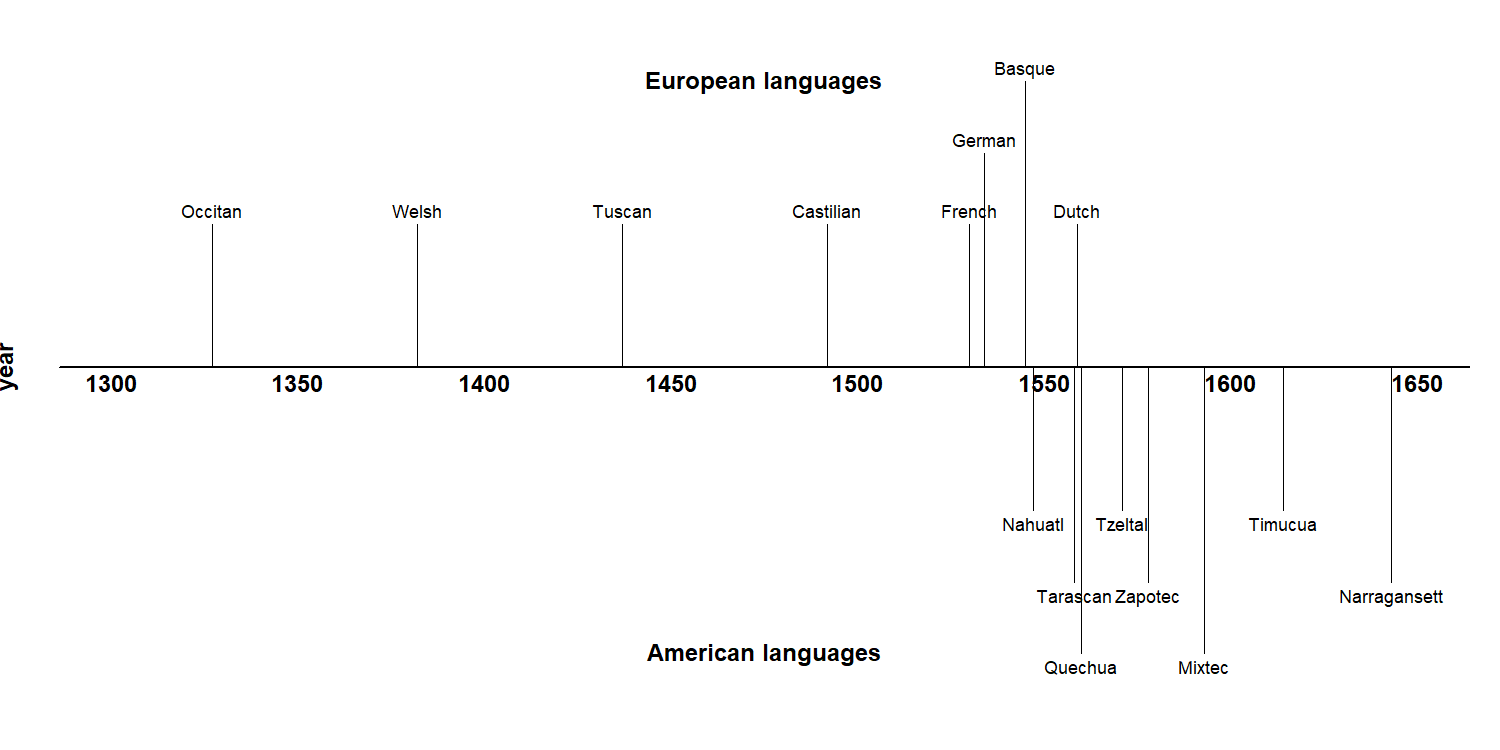
\includegraphics[width=\linewidth]{grammars.png}
  \caption{Approximate date of some of the first grammatical descriptions of European vs. American languages}
  \label{fig:grammars}
\end{figure}

\singlespacing
\setlength\LTleft{0pt}
\setlength\LTright{0pt}
\renewcommand{\arraystretch}{1.5}

\begin{longtable}{ l l l l }%
  \caption{Some first grammatical descriptions of European vs. American languages}
  \label{tab:grammars}\\
  \toprule
    Language     & Year       & Title                                                                                                                                                                                         & Author\\
  \midrule
  \endfirsthead
  \caption[]{Some first grammatical descriptions of European vs. American languages}\\
  \toprule
    Language     & Year       & Title                                                                                                                                                                                         & Author\\
  \midrule
  \endhead
    Irish        & 600s       & \parbox[t]{2.5in}{\pubtitle{Auraicept na n-Éces}\\\tln{The scholars' primer}}                                                                                                                 & Longarad\\
    Occitan      & 1327       & \parbox[t]{2.5in}{\pubtitle{Leys d'amors}\\\tln{Laws of love}}                                                                                                                                & Guilhèm Molinièr\\
    Welsh        & 1382--1410 & \parbox[t]{2.5in}{\pubtitle{Llyfr Coch Hergest}\\\tln{Red book of Hergest}}                                                                                                                   & unknown\\
    Tuscan       & 1437--1441 & \parbox[t]{2.5in}{\pubtitle{Grammatica della lingua toscana}\\\tln{Grammar of the Tuscan language}}                                                                                           & Leon Battista Alberti\\
    Castilian    & 1492       & \parbox[t]{2.5in}{\pubtitle{Gramática de la lengua castellana}\\\tln{Grammar of the Castilian language}}                                                                                      & Antonio de Nebrija\\
    French       & 1530       & \parbox[t]{2.5in}{\pubtitle{L'Éclaircissement de la langue francoyse}\\\tln{Explication of the French language}}                                                                              & John Palsgrave\\
    German       & 1534       & \parbox[t]{2.5in}{\pubtitle{Ein Teutsche Grammatica}\\\tln{A German grammar}}                                                                                                                 & Valentin Ickelsamer\\
    Basque       & 1545       & \parbox[t]{2.5in}{\pubtitle{Linguæ Vasconum Primitiæ}\\\tln{First fruits of the Basque language}}                                                                                             & Bernard Etxepare\\
    Totonac      & 1539--1554 & \parbox[t]{2.5in}{\pubtitle{Arte de la lengua totonaca}\\\tln{Grammar of the Totonac language}}                                                                                               & Andrés de Olmos\\
    Nahuatl      & 1547       & \parbox[t]{2.5in}{\pubtitle{Arte para aprender la lengua mexicana}\\\tln{Grammar for learning the Mexican language}}                                                                          & Andrés de Olmos\\
    Tarascan     & 1558       & \parbox[t]{2.5in}{\pubtitle{Arte de la lengua tarasca de Michoacán}\\\tln{Grammar of the Tarascan language of Michoacán}}                                                                     & Maturino Gilberti\\
    Dutch        & 1559       & \parbox[t]{2.5in}{\pubtitle{Den schat der Duytsscher Talen}\\\tln{The treasure of the Dutch language}}                                                                                        & John III van de Werve\\
    Quechua      & 1560       & \parbox[t]{2.5in}{\pubtitle{Grammatica o arte de la lengua general de los Indios de los Reynos del Peru}\\\tln{Grammar or Art of the General Language of the Indians of the Royalty of Peru}} & Domingo de Santo Tomás\\
    Tzeltal Maya & 1571       & \parbox[t]{2.5in}{\pubtitle{Ars Tzeldaica}\\\tln{Tzeltal Grammar}}                                                                                                                            & Fray Domingo de Hara\\
    Zapotec      & 1578       & \parbox[t]{2.5in}{\pubtitle{Arte en lengua Zapoteca}\\\tln{Grammar in the Zapotec language}}                                                                                                  & Juan de Córdova\\
    English      & 1586       & \parbox[t]{2.5in}{\pubtitle{Pamphlet for Grammar}}                                                                                                                                            & William Bullokar\\
    Mixtec       & 1593       & \parbox[t]{2.5in}{\pubtitle{Arte de lengua Mixteca}\\\tln{Grammar of the Mixtec language}}                                                                                                    & Antonio de los Reyes\\
    Timucua      & 1614       & \parbox[t]{2.5in}{\pubtitle{Gramatica de la lengua Timuquana de Florida}\\\tln{Grammar of the Timucua language of Florida}}                                                                   & Francisco Pareja\\
    Narragansett & 1643       & \parbox[t]{2.5in}{\pubtitle{A key into the language of America}}                                                                                                                              & Roger Williams\\
  \bottomrule
\end{longtable}

\renewcommand{\arraystretch}{1}
\doublespacing

As documentary linguistics turned its attention to North American (as opposed to Mesoamerican) languages, lexical flexibility in particular became a more prominent issue. In fact, even the first comprehensive survey of North American languages contains an entire section on \enquote{Conversion of nouns into verbs} \parencite[174--177]{Gallatin1836}, in which Gallatin depicts lexical flexibility as a rampant feature of all languages on the continent:

\blockquote[{\cite[175--176]{Gallatin1836}}]{It is the substantive [i.e. copula / auxiliary] verb which we [speakers of Indo-European languages] conjugate; whilst the [Native American] conjugates what we call the adjective and even the noun itself, in the same manner as [s/he] does other intransitive verbs. […] I believe it must appear sufficiently obvious, that this general if not universal character of the [Native American] languages, the conversion into verbs and the conjugation, through all the persons, tense, and moods, of almost all the adjectives and of every noun which, without a palpable absurdity, is suspectible of it, is entirely due to the absence of the substantive verb.}

As evidenced by the above passage, increasing familiarity with non-Indo-European languages prompted some writers to abandon the universalist commitment. However, categorial universalism is still a widely-held position today, either in the sense of a) being universally instantiated in all languages \parentext{commonly assumed by most generative frameworks; although see Culicover \parencite{Culicover1999}}, or b) being available to all languages, but only instantiated in some \parentext{sometimes called the \enquote{grab bag} approach, as exemplified by Dixon's Basic Linguistic Theory framework \parencite*[???]{Dixon2010a,b,c}; \parencites[???]{Hieber2013}[???]{Croft}}.

\subsection{Relativism}
\label{sec:2.2.2}

American ethnographers in the tradition of Franz Boas questioned the univeralist assumption in a programmatic and comprehensive way. Writing on grammatical categories, Boas states, \textquote[{\cite[35]{Boas1911}}]{Grammarians who have studied the languages of Europe and western Asia have developed a system of categories which we are inclined to look for in every language}. He concludes that this endeavor is a folly, and that \textquote[{\cite[35]{Boas1911}}]{in a discussion of the characteristics of various languages \qem{different fundamental categories} will be found}. Boas' students all adopted his grammatical relativism, and it became a foundational principle of the American linguistics tradition. His student Edward Sapir, writing on lexical categories specifically, makes one of the best-known and strongest statements of this position in his influential textbook \pubtitle{Language}: \textquote[{\cite[125]{Sapir1921}}]{[N]o logical scheme of the parts of speech—their number, nature, and necessary confines—is of the slightest interest to the linguist. Each language has its own scheme. Everything depends on the formal demarcations which it recognizes.}.

Many linguists today hold to Boas' grammatical relativism in some fashion or another. Textbooks and typological surveys commonly state that languages have varying numbers of lexical categories, though usually with the caveat that all languages seem to differentiate at least Noun and Verb \parencite[e.g.][§6.2]{Velupillai2012}. Some researchers, especially those working in typology, argue that linguists are still not rigorous \emph{enough} in their application of grammatical relativism; they criticize certain kinds of crosslinguistic comparisons for imposing the categories of one language onto another \parencites{Croft2001}{Haspelmath2010}{LaPolla2016} \addcite{You could probably cite your 2013 article for this too.}. This position is discussed further in \secref{sec:2.4}.

\subsection{Structuralism}
\label{sec:2.2.3}

Developing alongside the early anthropological linguistics of Boas was the linguistic structuralism of Ferdinand de Saussure. His work informed both the Prague school under Nikolay Trubetzkoy and Roman Jakobson, and the distributional method of Leonard Bloomfield. The term \dfn{structuralism} has any number of uses \parencite[Ch.~1]{Matthews2001}; here I refer to the idea that \textquote[{\cite[383]{Matthews2014}}]{language is a […] self-contained, self-regulating system, whose elements are defined by their relationship to other elements}. In particular, I am referring to the positivistic flavor of structuralism as practiced by Bloomfield, which focused on the structural relations between elements and establishing a set of rigorous scientific discovery procedures for linguistic structures \parencite{Bloomfield1933}. Bloomfield saw lexical categories as something to be empirically discovered in the different syntactic distributions of words, rather than imposed on a language a priori \parencite[33]{Rauh2010}. Zellig Harris later refined and expanded on this methodology \parencite{Harris1951}, which in turn was incorporated into Noam Chomsky's ealy Phrase Structure Grammar.

The signature methodological feature of this form of structuralism is the \dfn{distributional method}, a procedure for defining categories in terms of the set of contexts in which its words can appear—that is, their distributions \parencites[5]{Harris1951}[11]{Croft2001}. As an illustration of distributional analysis applied to lexical categories, \textcite[11--12]{Croft1991} considers the distributions of the \idx{English} words \txn{cold}, \txn{happy}, \txn{dance}, and \txn{sing} in two constructions: in the Predicate construction after \txn{be}, and in the \nth{3} Person Singular Present Tense (\txn{-s}) construction. Example data are shown below.

\begin{exe}
  \ex\label{ex:2.2}
    \begin{xlist}
      \setlength{\itemsep}{0em}
      \ex[]{Jack is cold.}
      \ex[*]{Jack colds.}
    \end{xlist}
  \ex\label{ex:2.3}
    \begin{xlist}
      \setlength{\itemsep}{0em}
      \ex[]{Jack is happy.}
      \ex[*]{Jack happies.}
    \end{xlist}
  \ex\label{ex:2.4}
    \begin{xlist}
      \setlength{\itemsep}{0em}
      \ex[*]{Jack is dance.}
      \ex[]{Jack dances.}
    \end{xlist}
  \ex\label{ex:2.5}
    \begin{xlist}
      \setlength{\itemsep}{0em}
      \ex[*]{Jack is sing.}
      \ex[]{Jack sings.}
    \end{xlist}
\end{exe}

We can see that \txn{cold} and \txn{happy} have the same distributions in these tests (both may appear in the Predicate construction but not the Person-Tense inflection construction), while \txn{dance} and \txn{sing} have the same distribution (the inverse situation as \txn{cold} and \txn{happy}). The results of these two distributional tests are summarized in \tabref{tab:English-distributions-a}.

\begin{table}[h]
  \centering
  \caption[Distribution of English Verbs and Adjectives]{Distribution of English Verbs and Adjectives \parentext{adapted from \textcite[12]{Croft2001}}}
  \label{tab:English-distributions-a}
  \begin{tabular}{ l c c }
    \toprule
      { } & \parbox{1in}{\centering Predicate{\newline}Construction} & \parbox{1in}{\centering Inflectional{\newline}Construction}\\
    \midrule
      \textbf{Adjective}: \txn{cold}, \txn{happy}, etc. & ✔ & ✘\\
      \textbf{Verb}:      \txn{sing}, \txn{dance}, etc. & ✘ & ✔\\
    \bottomrule
  \end{tabular}
\end{table}

As applied in practice, however, the distributional method suffers from one serious drawback when used to argue for large, traditional categories like noun, verb, and adjective: distributional tests yield conflicting and overlapping results. Perhaps no two lexical items behave the same in every distributional test. Each new test that is introduced therefore partitions the lexicon into smaller and smaller classes. This fact has been demonstrated empirically for French verbs \parencite{Gross1979}, Russian numerals \parencite{Corbett1978}, and English adjectives vs. adverbs \parencite[54]{Crystal1967}. Distributional tables like that in \tabref{tab:English-distributions-a} from each of these studies are reproduced in \tabref{tab:French-distributions}, \tabref{tab:Russian-distributions}, and \tabref{tab:English-distributions-b} respectively. It is clear from these studies that distributional analysis does \emph{not} lead to large, unified categories like noun, verb, and adjective, but rather a myriad of small constructions \parencite[434]{Croft2005}. This fact is the motivation underlying constructional approaches to language.

\TODO{add distributional tables}

Many scholars nonetheless choose to retain lexical categories as a necessary component of their linguistic theories or descriptions, at the expense of consistent application of the distributional method. Rather than considering all possible distributional contexts for a word, these scholars instead treat certain constructions as definitional of the category. Other distributional tests which yield cross-cutting results are either ignored, or treated as evidence of subcategories instead of categories. Many researchers even prefer the term \dfn{syntactic categories} over \dfn{lexical categories} for this reason, focusing on just the syntactic evidence for categories \addcite{Baker 2003; Rauh 2010}. A severe methodological problem for this approach is that there are no generally agreed-upon principles for determining which distributional tests should be considered definitional. In this regard, \textcite[4]{SchachterShopen2007} note, \textquote{there may be considerable arbitrariness in the identification of distinct parts of speech rather than subclasses}. Different scholars choose or prioritize different kinds of evidence for lexical categories over others on the basis of their theoretical commitments. This is the reason, as stated in \secref*{sec:1.1}, that disagreements about the existence of particular lexical categories in particular languages are typically \emph{not} about the empirical facts. The results of a given distributional analysis are not usually controversial; the choice of distributional tests used to support one's analysis are. Unsurprisingly, then, debates over how to analyze lexical categories in various languages have been largely unproductive and unresolved \parencite[435]{Croft2005}. The problem only worsens when scholars attempt to apply the same criteria across languages. Distributions of words with similar meanings vary drastically across languages \parencite[§1.4.1]{Croft2001}.

The real methodological problem here is \emph{not} that we have yet to ascertain the correct principles for selecting the right distributional tests. The problem is being selective regarding which tests to apply in the first place. If we take the distributional method seriously, then we must apply it consistently, without ignoring distributional evidence that contradicts our theoretical or pretheoretical assumptions. To do otherwise is a kind of \dfn{methodological opportunism} \addcite{Croft 1991: 10--15, 41 (check these pages); Croft 2001: ???}.

\TODO{add a section on mixed / hybrid categories (including Lois, Malouf, Nikolaeva)}

Partly in response to these problems, a growing cadre of linguists in the last 30 years have adopted one of various \dfn{flexible} approaches to word classes. Flexible analyses of word classes come in many flavors, some of which arguably still commit methodological opportunism, and others of which introduce new difficulties. These flexible approaches are reviewed in the following section.

\section{Flexible approaches}
\label{sec:2.3}

In this section I summarize the key concepts (\secref{sec:2.3.1}), findings (\secref{sec:2.3.2}), and criticisms (\secref{sec:2.3.2}) of lexical flexibility research. \secref*{sec:2.3.1} surveys the wide variety of definitions and theoretical perspectives on lexical flexibility. This review of the literature reveals that there is very little consensus as to what exactly constitutes \enquote{lexical flexibility}; as such, there are numerous alternative terms for the phenomenon. Despite these incongruities, a few important findings do consistently surface across the empirical research. These findings are summarized in \secref*{sec:2.3.2}. \secref*{sec:2.3.3} then looks at the arguments and evidence that researchers have presented against the notion of lexical flexibility.

\subsection{Key concepts}
\label{sec:2.3.1}

It is only a small exaggeration to say that there are as many definitions and terms for what I am here calling \enquote{lexical flexibility} as there are scholars who research it. I use the term \dfn{lexical flexibility} in this thesis merely because it is the most widely recognized of the cluster of terms that are used, not because it is necessarily the most precise or accurate. My own choice would be \dfn{functional expansion}, for reasons discussed below. The analytical or theoretical perspective adopted by each researcher generally determines their choice of terminology. The remainder of this section is devoted to explaining these perspectives in more detail.

Generally speaking, there are two ways to analyze flexible words. The first method assigns flexible words to members of specific categories in a language, whether those language-categories are the canonical four major classes (Noun, Verb, Adjective, Adverb), or a new large supercategory subsuming multiple discourse functions (e.g. contentives, non-verbs, flexibles), or a smaller subcategory of an existing major lexical category (e.g. adjective verbs, verbonominals). The second method of analysis assumes that words are uncategorized at some level (root, stem, or inflected word), and that words receive their categorial assignment from context. Different researchers posit different mechanisms for how words receive their categorization in context. The traditional approaches to lexical flexibility summarized in \secref*{sec:2.2} are all instances of the former method of analysis, while the flexible approaches outlined in this section are a mix of categorial and non-categorial analyses.

\subsubsection{Lexical flexibility}
\label{sec:2.3.1.1}

Though awareness of lexical flexibility can be traced back to at least \textcite[174--177]{Gallatin1836} if not earlier, the term \dfn{lexical flexibility} itself seems to have originated with \textcite[Ch.~4]{Hengeveld1992}. This publication, perhaps because it was the first to assign a technical term to the concept, marks a shift in how scholars frame the concept of lexical flexibility. Previously, the issue was framed in terms of whether particular languages (especially those of the Pacific Northwest) distinguished noun from verb \parencites{Kuipers1968}{Jacobsen1979}{Hebert1983}{Kinkade1983}{EijkHess1986}{JelinekDemers1994}. After this point, an increasing number of publications began to ask whether lexemes were \dfn{flexible} instead. Though the difference in emphasis seems subtle, this change constitutes a turning point because it fostered an increased interest in lexical flexibility as a grammatical phenomenon in its own right instead of just a problem for traditional categorization schemes.

Hengeveld's \citeyear[Ch.~4]{Hengeveld1992} typology of parts-of-speech systems is a whole-language typology wherein languages are either \dfn{specialized}, with one morphosyntactic category for each of the functions of reference (Noun), predication (Verb), referent modification (Adjective), and predicate modification (Adverb\footnote{Note that Hengeveld's typology only includes manner adverbs, not other semantic types of adverbs.}), or \dfn{non-specialized}. Non-specialized languages deviate from the four-category canon in one of two ways: one part of speech may assume more than one function with no additional morphosyntactic marking, in which case the language is considered \dfn{flexible}; or the language may lack a dedicated part of speech for that function entirely and use other, marked constructions instead, in which case the language is considered \dfn{rigid}.

\TODO{add examples of flexible vs. rigid languages, with explanations}

Hengeveld's analysis is of the categorial type discussed at the beginning of \secref*{sec:2.3.1}, specifically the supercategory kind. Each word is assumed to have a category, and new supercategories are introduced for words which have multiple functions: \dfn{contentives} for words which perform all four functions, \dfn{non-verbs} for words which perform all non-predicating functions, and \dfn{modifiers} for words words which perform referent modifier and predicate modifier functions.

Numerous scholars have since adopted Hengeveld's term \dfn{lexical flexibility} to describe cases where words serve more than one discourse function, regardless of their particular theoretical commitments or analysis of flexible words. As a convenient cover term, \dfn{lexical flexibility} is now well established.

\subsubsection{Polycategoriality}
\label{sec:2.3.1.2}

\textcite[4]{VapnarksyVeneziano2017} introduce the alternative term \dfn{polycategoriality} as their preferred characteriziation of flexible words. (The term is also used by \textcite{Carter2006}, but he does not give a precise definition for it.) While Vapnarksy \& Veneziano use this term mostly interchangeably with \dfn{lexical flexibility}, there are important differences between the two concepts. Hengeveld's use of \dfn{lexical flexibility} is meant to imply the existence of large, flexible supercategories that subsume multiple discourse functions, whereas Vapnarksy \& Veneziano are not committed to any particular schema for parts of speech. Central to their notion of polycategoriality is the idea that lexical categories exist, but that \textquote[{\cite[4]{VapnarksyVeneziano2017}}]{there are lexical forms that are not specified for lexical category (or are not specified fully, or univocally) on some level of representation.}. In other words, one word may belong simultaneously to multiple lexical categories. Under this definition, a language could still have all four major lexical categories but nonetheless exhibit rampant polycategoriality; this is not a possibility in Hengeveld's framework. Like Hengeveld, however, Vapnarksy \& Veneziano are committed to the existence of large lexical categories in particular languages. Their analysis is therefore also of the categorial kind discussed at the beginning of \secref*{sec:2.3.1}.

\subsubsection{Multifunctionality / Polyfunctionality}
\label{sec:2.3.1.3}

Another term for our phenomenon of interest, introduced by \parencite{Lier2012}, is \dfn{multifunctionality}, in which a single lexeme can have multiple discourse functions. An advantage of this analysis is that it takes no theoretical position on the issue of whether words are categorial or non-categorial; it focuses on just their functions. The term \dfn{multifunctionality} is meant to stand in contrast with \dfn{conversion} or \dfn{zero derivation}. van Lier takes \dfn{conversion} to be idiosyncratic and unproductive, producing meanings for words in alternate discourse functions that are not predictable (see \addcrossref{section on conversion} and \addcrossref{section on item-specific knowledge} for further discussion). Multifunctionality is also distinct from zero derivation from a common root. Instead, multifunctional words are those whose semantic interpretation is entirely predictable from context, and its uses in different contexts are productive. Its meaning should be \dfn{compositional} (see \addcrossref{section: criteria for flexibility > compositionality}). For example: when an action word is used in a referring construction its predicted meaning is that of an \dfn{action nominalization}, \tln{(the act of) X‑ing}; and when an object word is used in a predicate construction its predicted meaning is that of a \dfn{predicate nominal}, \tln{be an X}. Examples of these predictable, compositional meanings are shown in \addcrossref{EX and EX}.

\TODO{add examples of multifunctionality}

\noindent However, words used in their non-prototypical functions very frequently do not have predictable meanings. Consider the examples in \addcrossref{EX and EX}.

\TODO{add examples of conversion}

\TODO[caption = {add lead-out}]{Add lead-out explaining how the meanings of the latter examples are idiosyncratic and unpredictable.}

van Lier takes examples like those in \addcrossref{former examples} to be instances of genuine multifunctionality, and those in \addcrossref{latter examples} to be cases of conversion. Others have also adopted a position similar to van Lier's, in which only the semantically compositional / predictable uses of a word in different discourse functions are considered flexible \parencites[pages for compositionality criterion]{EvansOsada2005} \addcite{Croft 2005? Where he is critical of flexible analyses for ignoring idiosyncratic meanings}.

\subsubsection{Precategoriality / Acategoriality}
\label{sec:2.3.1.4}

The various approaches which analyze flexible words as being at some level uncategorized until they receive their interpretation from context may be lumped together under the umbrella terms \dfn{precategoriality} or \dfn{acategoriality}. Hopper \& Thompson's influential paper \citeyear{HopperThompson1984} is an early application of the concept of \dfn{acategoriality} to the analysis of flexible words:

\blockquote[{\cite[747]{HopperThompson1984}}]{[L]inguistic forms are in principle to be considered as \emph{lacking categoriality} completely unless nounhood or verbhood is forced on them by their discourse functions. To the extent that forms can be said to have an apriori existence outside of discourse, they are characterizable as \dfn{acategorial}; i.e. their categorical classification is irrelevant. Categoriality-the realization of a form as either a N or a V-is imposed on the form by discourse.}

The term \dfn{precategorial} has become a somewhat more common term for roughly the same concept (though some researchers use the term in more strictly-delineated ways) \parencites[357, 362--364]{EvansOsada2005}{Bisang2008a}{Bisang2008b}{Bisang2013}. It is especially preferred by morphological models that presuppose stages of derivation, such that words are precategorial before they reach a certain stage of the derivation \parencites{HalleMarantz1993}{Arad2005} \addcite{chapter from Handbook of morphological theory}. \textcite[5]{VapnarksyVeneziano2017} distinguish polycategoriality from acategoriality by defining acategoriality as implying \textquote{no primitive / original categorial marking at all}, and polycategoriality as allowing a form \textquote{to be only partially unspecified for category, with possible constraints on the relevant categories}. Languages for which precategorial analyses have been advanced include \idx{Cherokee} \parencite{Haag2017}, \idx{Gooniyandi} \parencite{McGregor2013}, \idx{Kuikuro} \parencite{FranchettoSantos2017}, Mundari \parencite{HengeveldRijkhoff2005}, and many others. \textcite{Pfeiler2006} also presents pscyholinguistic evidence that the earliest utterances of L1 learners of \idx{Yucatec Maya} are acategorial.

A central concern in precategorial approaches is the precise mechanism by which a word receives its categorization in context \parencite[Sec.~3.7]{HengeveldRijkhoffSiewierska2004}. There are two main theories of semantic indeterminacy in flexible words: \dfn{underspecificity} \parencites{Farrell2001}{RijkhoffLier2013} and \dfn{vagueness} \parencites{Tuggy1993}{HengeveldRijkhoffSiewierska2004}{HengeveldRijkhoff2005}. The essential difference is that underspecificity entails semantic minimalism while vagueness is entails semantic maximalism. An underspecified word has a minimal, core meaning, and receives its categorial meaning from the discourse context it appears in; a vague word has a maximal, broad meaning that covers all the possible discourse contexts it appears in. (There is of course quite a deal of variation in the literature as to how scholars use these terms, with many researchers conflating the two.) \textcite[414]{HengeveldRijkhoff2005} offer the example of \txn{cousin} as a word that is semantically underspecified for gender, such that the gender of the referent must be understood from context. \textcite{Denison2018} argues that the English word \txn{long} exhibits adjective {\textasciitilde} adverb underspecification in Old and Middle English.

In contrast, \textcite[539--541]{HengeveldRijkhoffSiewierska2004} outline a theory regarding exactly how vagueness operates in the context of lexical flexibility:

\blockquote[{\cite[541]{HengeveldRijkhoff2005}}]{[E]ach flexible lexeme has a single (vague) sense. By placing the flexible lexeme in a particular syntactic slot or by providing it with certain morphological markers, the speaker highlights those meaning components of the flexible lexeme that are relevant for a certain lexical (verbal, nominal, etc.) function. Thus we contend that the meaning of a flexible lexeme always remains the same, and that morphosyntactic and other contextual clues signal to the addressee how to interpret this lexeme in an actual utterance. In other words, it is the use of a vague lexeme in a certain context (an actual linguistic expression) that brings out certain parts of its meaning, giving the category-neutral lexeme a particular categorial (verbal, nominal, etc.) flavour.}

\noindent (Note that while vagueness implies a certain potential ambiguity, Hengeveld \& Rijkhoff reserve the term \dfn{ambiguity} for cases of distinct, homophonous words.)

\textcite[363--364]{EvansOsada2005} and \textcite{Kihm2017} criticize both precategorial approaches for their imprecision, claiming that it would be impossible to formulate a definition for many flexible words that was broad enough to encompass all their uses. \textcite[87]{Kihm2017} illustrates this difficulty with the various meanings of the \idx{Arabic} root \txn{s-q-t}, which could arguably be glossed \textsc{fall}. A selection of stems containing this root are given in \exref{ex:2.2}.

\TODO{add examples from Kihm (2017: 87)}

It is difficult to imagine a single definition of \txn{s-q-t} which could adequately demarcate just this set of meanings. This difficulty could perhaps be overcome, however, by loosening the requirement that the meaning of a word be unitary. Word meanings are \dfn{polycentric}, where different senses of a word are related through \dfn{meaning chains} rather than all through a single, central member \parencite[110]{Taylor2003}. This is sometimes referred to as a \dfn{family resemblance} structure for categories. The difference between monocentric and polycentric categories is illustrated schematically in \figref{fig:family-resemblance}. In both diagrams, each letter A–E represents a sense of a word. In the monocentric case, all the senses of the word are related through its core sense A. In the polycentric case, senses A and E are related only through their intervening connections.

\TODO[caption = {add diagram for monocentric vs. polycentric categories}]{Create a 2-part figure comparing monocentric vs. polycentric categories, with monocentric on the left. The senses in the monocentric case should be arranged circularly around sense A. The senses in the polycentric case should be arranged linearly from A > E.}

Recognizing that word meanings are polycentric addresses Evans \& Osada and Kihm's criticisms of vagueness theory because it shows that the disparate senses of a word can be related without having to share any core component of their meanings. The use of a lexeme in a certain context then profiles one of these senses over others. Kihm himself hints at this solution by referring to the related Arabic stems in \exref{ex:2.2} as a \dfn{lexical family}.

\subsection{Key findings}
\label{sec:2.3.2}

\subsubsection{Parts-of-speech hierarchy}
\label{sec:2.3.2.1}

Having outlined the concept of flexible languages, Hengeveld then presents the results of a 30-language survey of parts of speech in which he finds that the categories which are most likely to occur as an independent class in a language are subject to an implicational hierarchy, shown in \exref{ex:2.3}.

\begin{exe}
  \ex\label{ex:2.3} Verb > Noun > Adjective > Adverb
\end{exe}

\noindent Categories to the left of the hierarchy are more like to occur as a distinct part of speech than categories to the right. Applying this hierarchy to Hengeveld's flexible vs. rigid distinction yields the parts-of-speech typology in \figref{fig:Hengeveld-pos-systems} \parentext{adapted from \textcite[69]{Hengeveld1992} and \textcite[718]{Rijkhoff2007}}. The terms for the different categories in flexible languages are from \textcite{HengeveldRijkhoffSiewierska2004}. Hengeveld points out that this is not a strict classification scheme; languages may sit at the boundaries between types and exhibit exceptions.

\TODO[caption = {add parts-of-speech tables}]{parts of speech typology from Hengeveld \& Rijkhoff 2005: 407}

Hengeveld's parts-of-speech typology and the subsequent research it inspired \parencites{DonLier2003}{HengeveldRijkhoff2005}{Lier2006}{HengeveldLier2010}{Luuk2010}{LierRijkhoff2013}{Lier2016} constitute important empirical contributions to the study of lexical flexibility. However, Hengeveld's definition of flexible languages and his parts-of-speech typology still rely on large, language-specific categories of the kind that have been problematized by Croft \addcite{Croft's publications, especially the pages in 1991 where he critiques Hengeveld directly} and van Lier \parencite{CroftLier2012}, and are therefore subject to the same difficulties as traditional approaches to parts of speech. One could however reframe Hengeveld's implicational hierarchy in terms of functions rather than catgories, as in \exref{ex:2.3}.

\begin{exe}
  \ex\label{ex:2.3} predicate > referent > predicate modifier > referent modifier
\end{exe}

\noindent In \exref{ex:2.3}, functions to the left of the hierarchy are more likely to have dedicated morphosyntactic constructions than those to the right. This reformulation avoids a commitment to any language-particular categories while still capturing the important implicational trend observed by Hengeveld. As to Hengeveld's definition of lexical flexibility itself, I propose a revised, function-based definition in \secref*{sec:2.5} \parentext{see also \textcite[1]{LierRijkhoff2013} for a similar but more loosely-defined function-based definition}.

\subsubsection{Referent-predication asymmetries}
\label{sec:2.3.2.2}

\subsubsection{Locus of categoriality}
\label{sec:2.3.2.3}

\subsubsection{Item-specific flexibility}
\label{sec:2.3.2.4}

\subsubsection{Sense-specific flexibility}
\label{sec:2.3.2.5}

\subsection{Problems \& critiques}
\label{sec:2.3.3}

\section{Functional approaches}
\label{sec:2.4}

\subsection{Prototype theory}
\label{sec:2.4.1}

\subsection{Typological markedness theory}
\label{sec:2.4.2}

\section{Lexical flexibility: A functional definition}
\label{sec:2.5}
